\section{Problem Statement}

In the past couple of years, a vast inflow of retail and corporate capital has entered the cryptocurrency markets. As time goes by, one may notice a rising interest in these markets, as well as, an almost exponential increase in trading volumes. Although the cryptocurrency
market has many similarities with the traditional, the authors felt that the differences between them, are enough to differentiate their behavior from the traditional assets and thus investigation and research is deemed mandatory.

The approach the authors will take in this assignment is to analyze existing ideas and implement them on BTC timeseries, but at the same time, explore new approaches and combinations. The difficulty of this project lies with the asynchronous nature of information.
The way that information appear in the market must dictate the way they are represented, perceived by the researcher and used by a model. To illustrate this, we will use BTCUSD volume data, from Bitstamp exchange with index ranging from 2020-06-15 to 2020-09-15, aggregated weekly.

\begin{figure}[h]
	\centering
    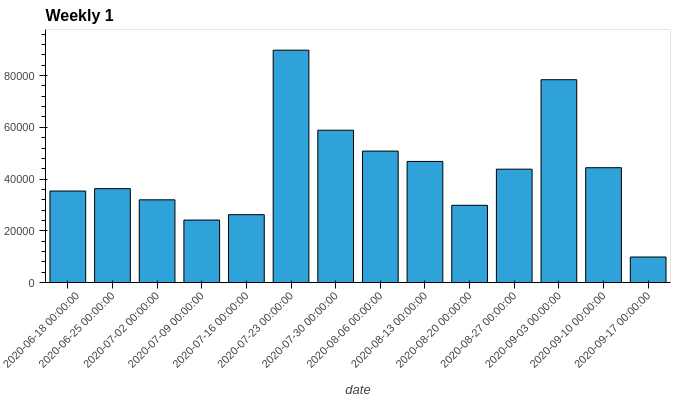
\includegraphics[width=6cm, height = 3.3cm]{one}
    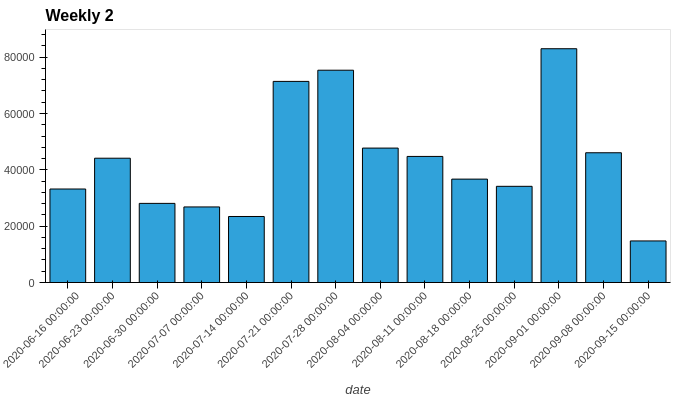
\includegraphics[width=6cm, height = 3.3cm]{two}
    \\[\smallskipamount]
    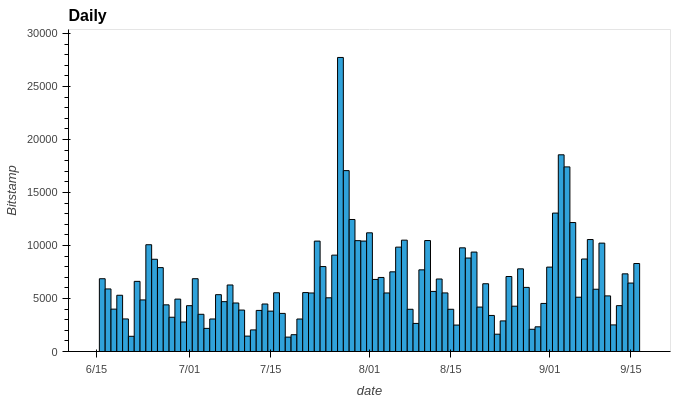
\includegraphics[width=6cm, height = 3.3cm]{three}
    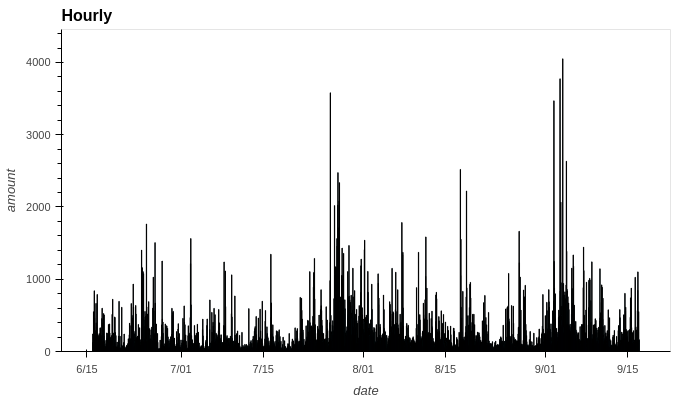
\includegraphics[width=6cm, height = 3.3cm]{four}
    \caption{BTCUSD Volume sampled in several timeframes}\label{fig:example}
\end{figure}


On the \textit{Weekly 1} chart, we observe that the week starting at 2020-07-23, has the biggest spike in volume across these 3 months while the next weeks exhibit declining volume. Another spike at
the week starting at 2020-09-03, also takes place. The \textit{Weekly 2} chart, is drawn on the same data, but before aggregating in weekly
timeframe (from daily), the dataset got shifted by 3 days to the left. As a result, the new chart is different from the previous one, as we observe
that the 2 week period that begins at 2020-07-21 had significant volume, but the highest spike now occurs at the week that starts 2020-09-08.

By changing the resolution to the daily timeframe, we observe that the volume that was attributed to two weeks in the previous graph, actually took place in 5 days, and the biggest spike in volume occurred in 2020-7-25. Further enhancing the resolution and aggregating to the hourly timeframe, the \textit{Hourly} chart,
shows a different story. There is a cluster of volume occuring at 2020-07-25 and persisting for
the week to come. More importantly, we observe a second spike around 2020-09-05 that is more pronounced but not as persistent (in terms of lags) as the first one.

\begin{figure}[h]
    \centering
    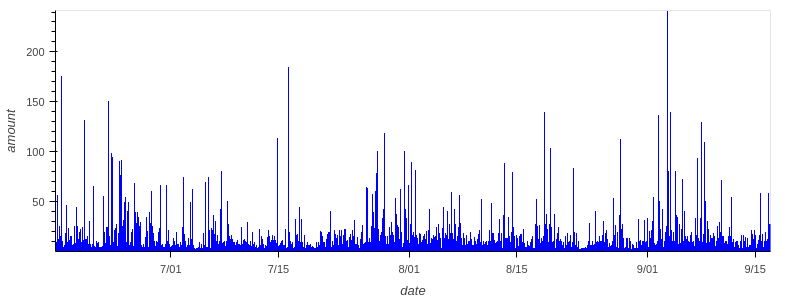
\includegraphics[width=10cm, height = 4cm]{five.png}
    \caption{Volume per trade (tick volume).}
    \label{fig:tick_vol}
\end{figure}

Lastly, the \ref{fig:tick_vol}, is the highest resolution possible and contains all the information we could possible get for volume in Bitstamp during that period. This chart, looks more like a series of impulses (sudden spikes) while some clusters of volume can be seen on the bottom of the graph (it is produced using the \textit{rasterize} method where a graph is treated as an image, therefore, it is impossible to visually assess how strong a cluster might be). 

What a researcher and an algorithm might extract from the above data, could be different in
each occasion, nevertheless, it is the same data (except for the 3 days shift that illustrate the danger of sampling in large timeframes), containing the same information. The above example used different fixed timeframe intervals but the same applies to sampling based on the side of the trade, or the number of trades. 

So, why not always use the highest resolution possible, in order to preserve all the information? This question leads us to the next tradeoff: The lower the resolution, the more information is lost, and the higher it is, the more noisy and less useful the data become.

The above example illustrates the main drive of this project: the necessity for proper sampling in high frequency data. This project, will opt to overcome this problem by sampling asynchronously and
dynamically, on the same dataset and across different features.


